\documentclass{beamer}

\usepackage{graphicx}
\usepackage[latin1]{inputenc}
\usepackage[T1]{fontenc}
\usepackage[english]{babel}
\usepackage{listings}
\usepackage{xcolor}
\usepackage{eso-pic}
\usepackage{mathrsfs}
\usepackage{url}
\usepackage{amssymb}
\usepackage{amsmath}
\usepackage{multirow}
\usepackage{hyperref}
\usepackage{booktabs}
% \usepackage{bbm}
\usepackage{cooltooltips}
\usepackage{colordef}
\usepackage{beamerdefs}
\usepackage{lvblisting}

\usepackage{multimedia}
\usepackage{algorithmicx}
\usepackage[noend]{algpseudocode}
\usepackage{algorithm}

\pgfdeclareimage[height=2cm]{logobig}{hulogo}
\pgfdeclareimage[height=0.7cm]{logosmall}{Figures/LOB_Logo}

\renewcommand{\titlescale}{1.0}
\renewcommand{\titlescale}{1.0}
\renewcommand{\leftcol}{0.6}

\title[Eigenvalue Problems - Numerical Solutions]{Eigenvalues and Eigenvectors}
\authora{Thomas Siskos}
\authorb{}
\authorc{}

\def\linka{siskosth@student.hu-berlin.de}
\def\linkb{http://github.com/thsis/NIS18}
\def\linkc{}

\institute{Numerical Introductory Seminar \\
Humboldt--University Berlin \\}

\hypersetup{pdfpagemode=FullScreen}

\begin{document}

% 0-1
%%%%%%%%%%%%%%%%%%%%%%%%%%%%%%%%%%%%%%%%
\frame[plain]{

\titlepage
}

\frame{
  \frametitle{Agenda}
  \tableofcontents
}
%%%%%%%%%%%%%%%%%%%%%%%%%%%%%%%%%%%%%%%%
\section{Motivation}
%%%%%%%%%%%%%%%%%%%%%%%%%%%%%%%%%%%%%%%%

% 1-1
%%%%%%%%%%%%%%%%%%%%%%%%%%%%%%%%%%%%%%%%
\frame[containsverbatim]{
\frametitle{PCA}
\begin{columns}[onlytextwidth]
\begin{column}{0.25\textwidth}
	\begin{itemize}
		\item The iris dataset is already linearly separable.
		\item With various techniques we can show this in even more detail.
	\end{itemize}
\end{column}
\begin{column}{0.75\textwidth}
	\begin{center}
	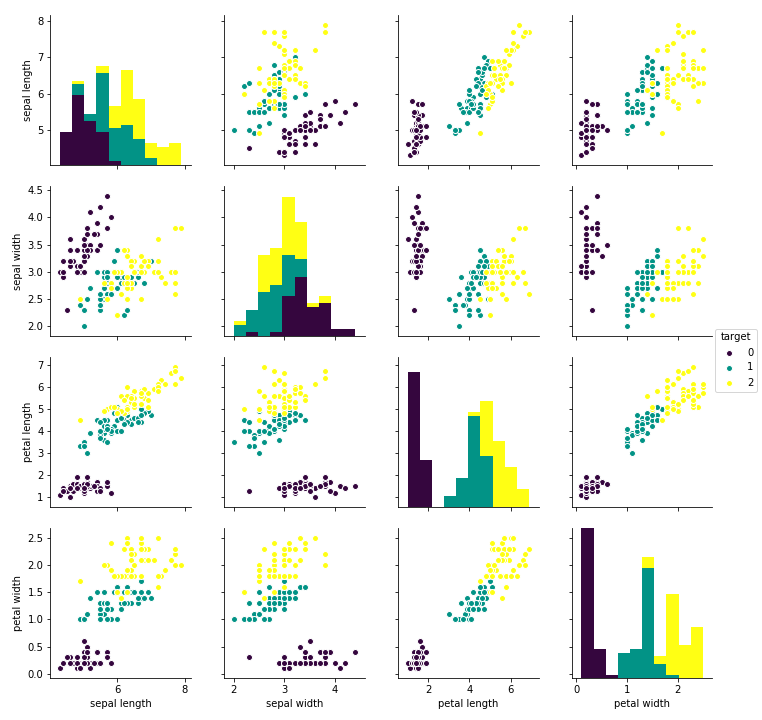
\includegraphics[scale=0.20]{../media/plots/iris_raw.png}
	\end{center}

\end{column}
\end{columns}
}
\frame[containsverbatim, label=PCA-prop]{
\frametitle{PCA}
\begin{columns}[onlytextwidth]
\begin{column}{0.65\textwidth}
	\begin{itemize}
		\item objective:
		\begin{equation}
		\label{pca_obj}
            max\ \delta^{\prime} Var \left(X\right) \delta \; s.t. \; \sum \delta_i^2 = 1.
        \end{equation}
        where $X \in \mathbb{R}^{n \times m}; m,n \in \mathbb{N}; \delta \in \mathbb{R}^m$
		\item solution \hyperlink{PCA-proof}{\beamergotobutton{Proof}}
:
		\begin{equation}
		\label{pca_sol}
			Y = \Gamma^{\prime} \left(X - \mu\right)
		\end{equation}
		where $Y \in \mathbb{R}^{n \times m}$ is the matrix of rotations, 
		      $\Gamma \in \mathbb{R}^{m \times m}$ is the matrix of eigenvectors,
		      $\mu \in \mathbb{R}^m$ is the vector of sample means.
	\end{itemize}
\end{column}
\begin{column}{0.35\textwidth}
	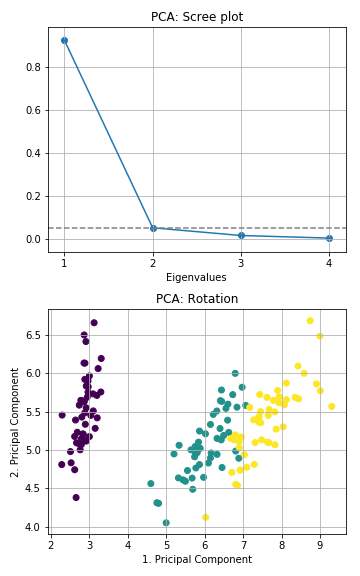
\includegraphics[width=3.5cm, height=6.5cm]{../media/plots/iris_pca.png}
\end{column}
\end{columns}
}

\frame{
\frametitle{LDA}
\begin{itemize}
	\item objective:
		\begin{equation}
		\label{lda_obj}
  			max \ \frac{w^{\prime}S_B w}{w^{\prime}S_W w},
		\end{equation}
	where 
	\begin{align*}
  	S_B &= \sum\limits_{c}^{C} (\mu_c - \mu)(\mu_c - \mu)^{\prime}, \\
  	S_W &= \sum\limits_{c}^{C} \sum\limits^{n}_{i=1} (x_i - \mu_c)(x_i - \mu_c)^{\prime}
	\end{align*}
	and $x_i \in \mathbb{R}^m$, $\mu_c$ is the vector of class means.
\end{itemize}

}

\frame[containsverbatim]{
\frametitle{LDA}
\begin{columns}[onlytextwidth]
\begin{column}{0.65\textwidth}
\begin{itemize}
\item solution \hyperlink{LDA-proof}{\beamergotobutton{Proof}}:
\begin{equation}
  \label{lda_sol}
    S_B^{-\frac{1}{2}}S_{W}^{-1}S_B^{-\frac{1}{2}} w = \lambda w
  \end{equation}
  where this is again an Eigenvalue problem and it's solution will provide the rotation that ensures the largest possible (linear) separability.
\item Now how do we get the Eigenvalues?
\end{itemize}
\end{column}
\begin{column}{0.35\textwidth}
	\begin{center}
	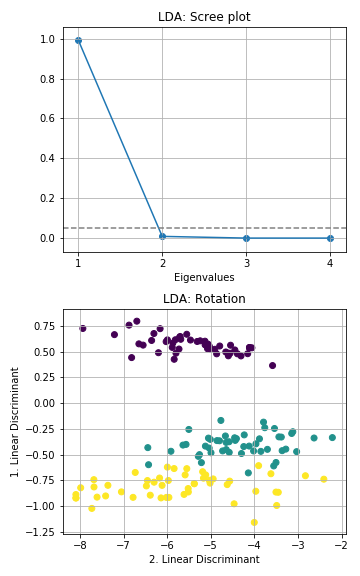
\includegraphics[width=3.5cm, height=6.5cm]{../media/plots/iris_lda.png}
	\end{center}
\end{column}
\end{columns}

}

\section{Key Idea \& Definitions}
\frame{
\frametitle{}

}
\subsection{Characteristic Polynomial \& Diagonal Matrices}
\frame{

}
\subsection{Similarity Transformations}
\subsubsection{Householder Reflections}
\subsubsection{Givens Rotations}

\section{Algorithms}
\subsection{Jacobi-Method}
\frame{

}

\frame{
\frametitle{Jacobi-Method}
\begin{algorithm}[H]
\caption{\texttt{jacobi}}
\label{j-meth}
\begin{algorithmic}
  \Require symmetric matrix $A$
  \Ensure $0 < precision < 1$
  \Statex \textbf{initialize: } $L \gets A$; $U \gets I$; $L_{max} \gets 1$
  \While{$L_{max} > precision$}
    \State Find indices $i$, $j$ of largest value in lower triangle of $abs(L)$
        \State $L_{max} \gets L_{i,j}$
            \State $\alpha \gets \frac{1}{2}\cdot \arctan(\frac{2A_{i, j}}{A_{i, i}-A_{j, j}})$
    \State $V \gets I$
    \State $V_{i, i}, V_{j, j} \gets \cos \alpha$; $V_{i, j}, V_{j, i} \gets -\sin \alpha, \sin \alpha$
    \State $A \gets V^{\prime} A V$; $U \gets UV$

  \EndWhile
  \Return $diag(A), U$
\end{algorithmic}
\end{algorithm}
}
\subsection{QR-Method}
\frame{

}

\subsubsection{Basic Variant}
\frame{
\frametitle{Basic QR-Method}
\begin{algorithm}[H]
\caption{\texttt{QRM1}}
\label{qr1-meth}
  \begin{algorithmic}
    \Require square matrix $A$
    \Statex \textbf{initialize: } $conv \gets False$
    \While{not $conv$}
      \State $Q, R \gets$ QR-Factorization of $A$
      \State $A \gets RQ$
      \If{$A$ is diagonal}
        \State $conv \gets \texttt{True}$
        \Statex
      \EndIf
    \EndWhile
    \Return $diag\left(A\right), Q$
  \end{algorithmic}
\end{algorithm}
}
\subsubsection{Hessenberg Variant}
\frame{
\frametitle{Refined QR-Method}
\begin{algorithm}[H]
\caption{\texttt{QRM2}}
\label{qr2-meth}
\begin{algorithmic}
  \Require square matrix $A$
  \State $A \gets \texttt{hessenberg(}A\texttt{)}$
  \State continue with: \Call {QRM1} A
\end{algorithmic}
\end{algorithm}
}

\frame{
  \frametitle{QRM2 Visualized}
  \begin{center}
    \movie[width=8cm, height=5.35cm]{\includegraphics[width=8cm, height=5.35cm]{Figures/placeholder.jpg}}{Figures/qrm_symmetric.mp4}
  \end{center}
}
\subsubsection{Accelerated Variant}
\frame{
\frametitle{Accelerated QR-Method}
\begin{algorithm}[H]
\begin{algorithmic}
\Require square matrix $A$
\end{algorithmic}
\end{algorithm}
}


\section{Analysis}
\subsection{Accuracy}
\frame{

}
\subsection{Efficiency}
\frame{
\frametitle{Time taken}
\begin{center}
  
\includegraphics[width=11.5cm, height=6cm]{../media/plots/time_boxplot.png}
\end{center}
}
\frame{
\frametitle{Iterations needed}
\begin{center}
  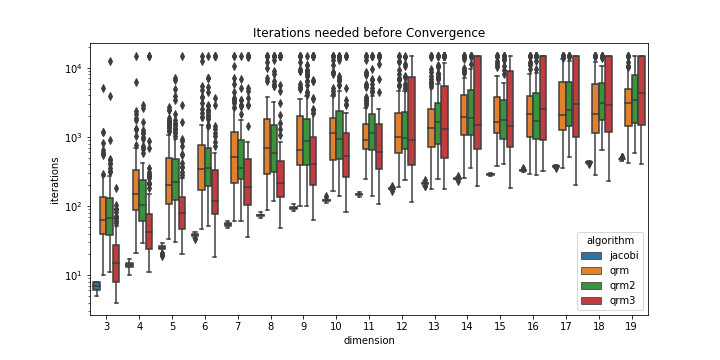
\includegraphics[width=11.5cm, height=6cm]{../media/plots/iterations_boxplot.png}
\end{center}
}



\frame[label=PCA-proof]{
\frametitle{PCA: proof}
The objective of \hyperlink{PCA-prop}{\beamergotobutton{PCA}}:
	$$
	max\ \delta^{\prime} Var \left(X\right) \delta \; s.t. \; \sum \delta_i^2 = 1
	$$
Corresponding Lagrangean:
    $$
    \mathcal{L}(Var \left(X\right), \delta, \lambda) = 
    \delta^{\prime} Var \left(X\right) \delta - \lambda \left(\delta^{\prime}\delta - 1\right),
    $$
    where $\lambda \in \mathbb{R}^m$ \\
First order condition:
	\begin{align}
	\frac{\partial \mathcal{L}}{\partial \delta} &\stackrel{!}{=} 0 \notag\\
	2Var(X)\delta - 2\lambda_k \delta &\stackrel{!}{=} 0 \notag\\
	Var(X)\delta  &= \lambda_k \delta \notag
	\end{align}
Which is now reduced to a common Eigenvalue problem.
}

\frame[label=LDA-proof]{
\frametitle{LDA: proof}
The objective of \hyperlink{LDA-prop}{\beamergotobutton{LDA}}:
  $$ max \ \frac{w^{\prime}S_B w}{w^{\prime}S_W w},$$
Which we can reformulate to:
  $$ max w^{\prime}S_B w \ s.t. w^{\prime}S_W w = 1. $$
Corresponding Lagrangean:
  $$ \mathcal{L}(w, S_B, S_W, \lambda) = w^{\prime}S_B w - \lambda \left(w^{\prime}S_W w - 1\right)$$
}
\frame{
\frametitle{LDA: proof}
First order condition:
\begin{align*}
\frac{\partial \mathcal{L}}{\partial w} &\stackrel{!}{=} 0 \notag \\
2S_B w - 2 \lambda S_W w &\stackrel{!}{=} 0 \notag \\
S_{W}^{-1}S_B w &= \lambda w, \\
\end{align*}
which is known as a generalized Eigenvalue problem. We can also rewrite this as:
$$S_B^{-\frac{1}{2}}S_{W}^{-1}S_B^{-\frac{1}{2}} w = \lambda w$$

Which is a now just a normal Eigenvalue problem as before \hyperlink{LDA-prop}{\beamergotobutton{back}}.
}

\end{document}
